\documentclass[10pt]{book}

%These tell TeX which packages to use.
\usepackage{array,epsfig}
\usepackage{amsmath}
\usepackage{amsfonts}
\usepackage{amssymb}
\usepackage{amsxtra}
\usepackage{amsthm}
\usepackage{mathrsfs}
\usepackage{color}
\usepackage{enumitem}
%\usepackage{mdframed}
\usepackage[most]{tcolorbox}
\usepackage{pgfplots}
\pgfplotsset{compat=1.6}

\pgfplotsset{soldot/.style={color=black,only marks,mark=*}} \pgfplotsset{holdot/.style={color=black,fill=white,only marks,mark=*}}

%Here I define some theorem styles and shortcut commands for symbols I use often
\theoremstyle{definition}
\newtheorem{defn}{Definition}
\newtheorem{thm}{Theorem}
\newtheorem{cor}{Corollary}
\newtheorem*{rmk}{Remark}
\newtheorem{lem}{Lemma}
\newtheorem*{joke}{Joke}
\newtheorem{ex}{Example}
\newtheorem*{soln}{Solution}
\newtheorem{prop}{Proposition}

\newcommand{\lra}{\longrightarrow}
\newcommand{\ra}{\rightarrow}
\newcommand{\surj}{\twoheadrightarrow}
\newcommand{\graph}{\mathrm{graph}}
\newcommand{\bb}[1]{\mathbb{#1}}
\newcommand{\Z}{\bb{Z}}
\newcommand{\Q}{\bb{Q}}
\newcommand{\R}{\bb{R}}
\newcommand{\C}{\bb{C}}
\newcommand{\N}{\bb{N}}
\newcommand{\M}{\mathbf{M}}
\newcommand{\m}{\mathbf{m}}
\newcommand{\MM}{\mathscr{M}}
\newcommand{\HH}{\mathscr{H}}
\newcommand{\Om}{\Omega}
\newcommand{\Ho}{\in\HH(\Om)}
\newcommand{\bd}{\partial}
\newcommand{\del}{\partial}
\newcommand{\bardel}{\overline\partial}
\newcommand{\textdf}[1]{\textbf{\textsf{#1}}\index{#1}}
\newcommand{\img}{\mathrm{img}}
\newcommand{\ip}[2]{\left\langle{#1},{#2}\right\rangle}
\newcommand{\inter}[1]{\mathrm{int}{#1}}
\newcommand{\exter}[1]{\mathrm{ext}{#1}}
\newcommand{\cl}[1]{\mathrm{cl}{#1}}
\newcommand{\ds}{\displaystyle}
\newcommand{\vol}{\mathrm{vol}}
\newcommand{\cnt}{\mathrm{ct}}
\newcommand{\osc}{\mathrm{osc}}
\newcommand{\LL}{\mathbf{L}}
\newcommand{\UU}{\mathbf{U}}
\newcommand{\support}{\mathrm{support}}
\newcommand{\AND}{\;\wedge\;}
\newcommand{\OR}{\;\vee\;}
\newcommand{\Oset}{\varnothing}
\newcommand{\st}{\ni}
\newcommand{\wh}{\widehat}
%Pagination stuff.
\setlength{\topmargin}{-0.75in}
\setlength{\oddsidemargin}{0in}
\setlength{\evensidemargin}{0in}
\setlength{\textheight}{9.in}
\setlength{\textwidth}{6.5in}
\pagestyle{empty}
\begin{document}
\begin{flushleft}
Name:\underline{\hspace{13cm}}Date:\underline{\hspace{2cm}}
\end{flushleft}
\begin{center}
{\Large Math 1041-012 \hspace{0.5cm} Section 2.1: Tangent \& Velocity}
\end{center}
%\vspace{0.2 cm}

\begin{tcolorbox}
\subsection*{Big Calculus Problem!}
\begin{enumerate}
    \item \textbf{Tangent Problem}: At a given point on any curve, how to find the equation of the tangent line??
    \item \textbf{Velocity Problem}: How do we compute the \textit{instantaneous rate of change} given the position function of an object??
\end{enumerate}
\textbf{SLOPE-INTERCEPT}:\\[4PT] \\
\textbf{POINT-SLOPE}: \\ [4PT]
\end{tcolorbox}

\subsection*{Example 1: Find an equation of the tangent line!}
Find an equation of the tangent line to the parabola $y=x^2$ at the point $P(1,1)$.
\begin{figure}[h!]
    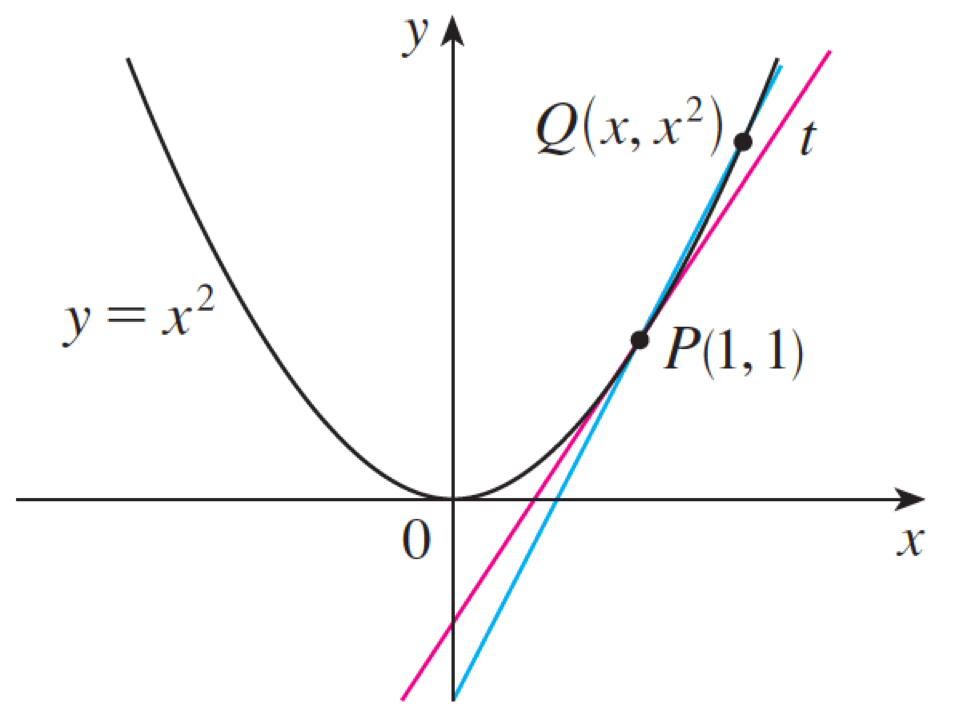
\includegraphics[scale=0.4]{fig1.png}
\end{figure}
\begin{figure}[h!]
    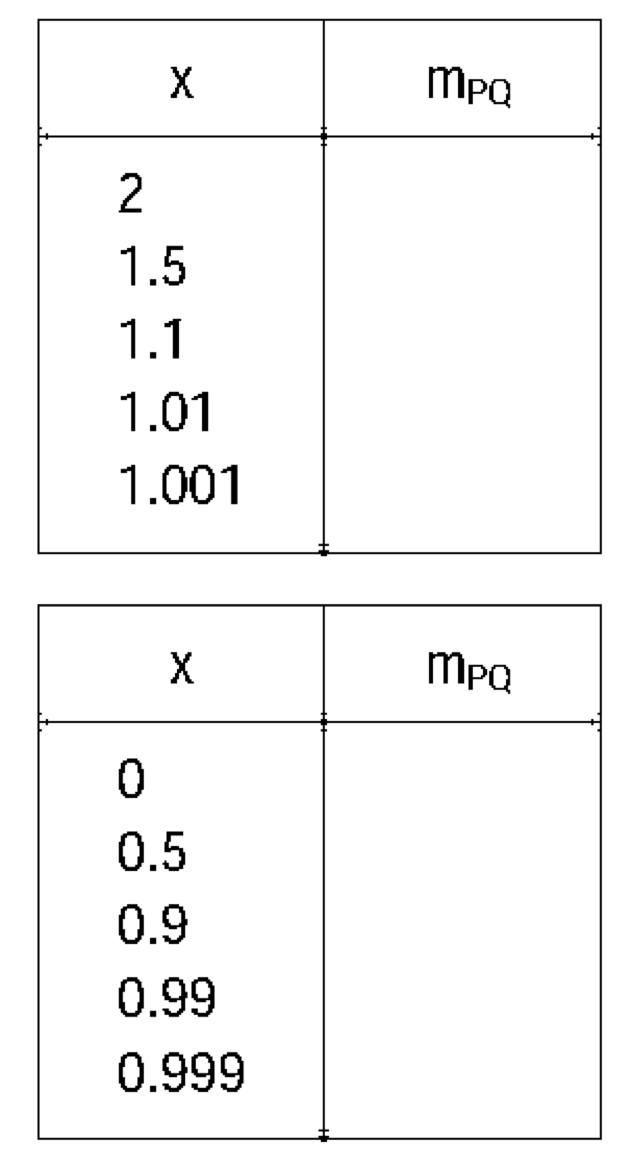
\includegraphics[scale=0.35]{fig2.png}
\end{figure}
\clearpage
\subsection*{Example 2: Velocity Problem}
Suppose that a ball is dropped from the upper observation deck of the CN Tower in Toronto, 450 meters above the ground. Find the velocity of the ball after 5 seconds. The position of the ball as it falls is given by $s(t)=4.9t^2$.\\
\begin{tcolorbox}
\subsection*{Velocity Problem}
\begin{itemize}
    \item We are finding instantaneous rate of change at a point!
    \item So far all we have is average rate of change
    \[
    AVE.\ RATE\ CHANGE = v_{ave}=\frac{change\ position}{change\ time}=\frac{\Delta s}{\Delta t}=\frac{s(t_1)-s(t_0)}{t_1-t_0}
    \]
    \item But as we shrink the change in time: $\Delta t\rightarrow 0 $ then
    \[
    \lim_{\Delta t\rightarrow 0 }v_{ave}=v_{inst}
    \]
\end{itemize}
\end{tcolorbox}
\begin{enumerate}
    \item[(a)] Find the average velocity for the time period beginning when $t=5$ and lasting $1$ second.\vspace{2cm}
    \item[(b)]Find the average velocity for the time period beginning when $t=5$ and lasting $0.1$ seconds.\vspace{2cm}
    \item[(c)] Find the average velocity for the time period beginning when $t=5$ and ending at $5.05$ seconds.\vspace{2cm}
    \item[(d)] What is the velocity of the ball after 5 seconds??
    \begin{figure}[h!]
        \centering
        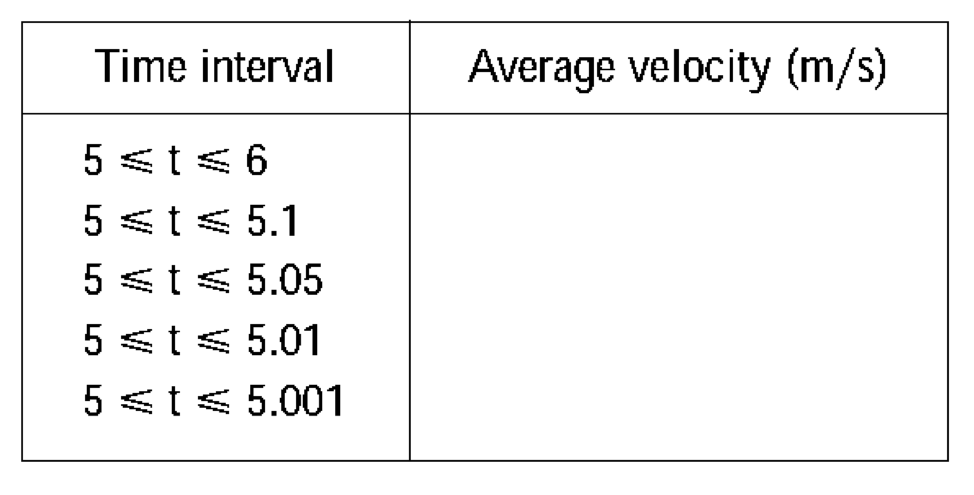
\includegraphics[scale=0.5]{fig3.png}
    \end{figure}
\end{enumerate}
\clearpage
\end{document}